\documentclass[aspectratio=169,10pt]{beamer}
\usetheme{Madrid}
\usecolortheme{default}

\usepackage{hyperref}
\usepackage{tikz}
\usetikzlibrary{patterns,shapes,arrows,calc,positioning,decorations.markings}
\usepackage{circuitikz}
\usepackage{amsmath,amssymb}
\usepackage{graphicx}
\usepackage{listings}
\usepackage{booktabs}

% --- Custom Colors UNIB ---
\definecolor{unibblue}{RGB}{0, 32, 96}
\definecolor{unibgold}{RGB}{197, 160, 89}
\definecolor{unibgreen}{RGB}{34, 112, 60}

\setbeamercolor{palette primary}{bg=unibblue,fg=white}
\setbeamercolor{palette secondary}{bg=unibblue!85,fg=white}
\setbeamercolor{palette tertiary}{bg=unibblue!70,fg=white}
\setbeamercolor{structure}{fg=unibblue}
\setbeamercolor{titlelike}{parent=structure,bg=unibblue,fg=white}
\setbeamercolor{block title}{bg=unibblue!90,fg=white}
\setbeamercolor{block body}{bg=unibblue!8,fg=black}
\setbeamercolor{alertblock title}{bg=unibgold!95,fg=black}
\setbeamercolor{alertblock body}{bg=unibgold!15,fg=black}
\setbeamercolor{exampleblock title}{bg=unibgreen!90,fg=white}
\setbeamercolor{exampleblock body}{bg=unibgreen!10,fg=black}

% --- Pengaturan Listing Julia ---
\lstdefinelanguage{Julia}%
  {morekeywords={abstract,break,case,catch,const,continue,do,else,elseif,%
      end,export,false,for,function,global,if,import,%
      let,local,macro,module,mutable,primitive,quote,return,struct,%
      true,try,type,using,var,while},%
   sensitive=true,%
   morecomment=[l]{\#},%
   morecomment=[n]{\#=}{=\#},%
   morestring=[b]',%
   morestring=[b]"%
  }[keywords,comments,strings]

\lstdefinestyle{juliastyle}{
    language=Julia,
    basicstyle=\ttfamily\tiny,
    keywordstyle=\color{blue!80!black}\bfseries,
    commentstyle=\color{green!50!black}\itshape,
    stringstyle=\color{red!80!black},
    numbers=none,
    breaklines=true,
    showstringspaces=false,
    frame=single,
    backgroundcolor=\color{gray!6},
    xleftmargin=4pt,
    xrightmargin=4pt,
    aboveskip=2pt,
    belowskip=2pt
}

\title[Persamaan Diferensial (Minggu 1)]{Persamaan Diferensial}
\subtitle{Minggu 1: Klasifikasi PDB/PDP, Nilai Awal (IVP), \& Pemodelan Fisis RL}
\author[Novalio \& Arfan (UNIB)]{Ir. Novalio Daratha, S.T., M.Sc., Ph.D. \& Muhammad Arfan, S.T., M.T.}
\institute[Teknik Elektro UNIB]{Program Studi S1 Teknik Elektro, Jurusan Teknik Elektro \& Informatika\\Fakultas Teknik, Universitas Bengkulu}
\date[2026]{Semester Genap 2026}

\begin{document}

% FRAME 1: Titlepage
\begin{frame}[plain]
  \titlepage
\end{frame}

% FRAME 2: Sub-CPMK OBE Bloom
\begin{frame}{Capaian Pembelajaran (Sub-CPMK) \& Taksonomi Bloom}
  \begin{block}{Sub-CPMK Minggu 1 (OBE Terintegrasi)}
    Mahasiswa mampu mengidentifikasi, mengklasifikasi, dan memodelkan fenomena dinamika sistem elektrik terpusat ke dalam Persamaan Diferensial Biasa (PDB) orde 1 serta memvalidasinya secara numerik.
  \end{block}
  \vspace{0.2cm}
  \begin{columns}[t]
    \column{0.5\textwidth}
    \textbf{Target Kognitif (Bloom C1--C3):}
    \begin{itemize}
      \item \textbf{C1 (Mengingat):} Menyebutkan definisi PDB, PDP, orde, derajat, dan syarat linieritas.
      \item \textbf{C2 (Memahami):} Membedakan solusi umum vs solusi khusus melalui syarat awal (IVP).
      \item \textbf{C3 (Menerapkan):} Menurunkan model KVL sirkuit RL menjadi PDB standar.
    \end{itemize}

    \column{0.5\textwidth}
    \textbf{Target Kognitif (Bloom C4--C6):}
    \begin{itemize}
      \item \textbf{C4 (Menganalisis):} Menganalisis evolusi transien berdasarkan konstanta waktu $\tau = L/R$.
      \item \textbf{C5 (Mengevaluasi):} Memvalidasi solusi analitik dengan komputasi numerik Julia.
      \item \textbf{C6 (Merancang):} Menaksir parameter sirkuit proteksi kumparan pemutus daya (PMT).
    \end{itemize}
  \end{columns}
\end{frame}

% FRAME 3: Peta Jalan Kurikulum & Intuisi Fisika
\begin{frame}{Peta Jalan Kurikulum \& Filosofi Dinamika Elektro}
  \begin{columns}[c]
    \column{0.52\textwidth}
    \textbf{Mengapa Persamaan Diferensial?}
    \begin{itemize}
      \item Hukum fisika elektro bekerja pada \textbf{laju perubahan}:
      \begin{equation*}
        i_C(t) = C \frac{dv_C}{dt}, \quad v_L(t) = L \frac{di_L}{dt}
      \end{equation*}
      \item Resistor mendisipasikan kalor ($R i^2$), sedangkan $L$ dan $C$ menyimpan energi medan ($\frac{1}{2} L i^2$ dan $\frac{1}{2} C v^2$).
      \item Keseimbangan energi menghasilkan \textbf{persamaan diferensial}.
    \end{itemize}

    \column{0.44\textwidth}
    \begin{block}{Dua Pilar Kurikulum PD Elektro}
      \textbf{Paruh 1 (Minggu 1--7):}
      PDB Orde 1 \& 2, Resonansi RLC, dan Transformasi Laplace $\rightarrow$ \textit{Analisis Transien Sirkuit}.
      \vspace{0.15cm}

      \textbf{Paruh 2 (Minggu 9--15):}
      PDP, Deret Fourier, Gelombang Telegrafer, \& Persamaan Maxwell $\rightarrow$ \textit{Medan Elektromagnetika}.
    \end{block}
  \end{columns}
\end{frame}

% FRAME 4: PDB vs PDP
\begin{frame}{Taksonomi Persamaan Diferensial: PDB vs PDP}
  \begin{columns}[t]
    \column{0.5\textwidth}
    \begin{block}{PDB (Ordinary Differential Equations)}
      Mengandung turunan dari satu atau lebih variabel tak bebas terhadap \textbf{satu variabel bebas tunggal} ($t$).
      \vspace{0.1cm}
      \begin{itemize}
        \item Karakteristik: Sistem parameter terpusat (\textit{lumped parameter systems}).
        \item Contoh Rangkaian RC:
        \begin{equation*}
          R C \frac{dv_C(t)}{dt} + v_C(t) = V_s(t)
        \end{equation*}
        \item Contoh Osilator RLC:
        \begin{equation*}
          L \frac{d^2 i(t)}{dt^2} + R \frac{di(t)}{dt} + \frac{1}{C} i(t) = 0
        \end{equation*}
      \end{itemize}
    \end{block}

    \column{0.5\textwidth}
    \begin{exampleblock}{PDP (Partial Differential Equations)}
      Mengandung turunan parsial terhadap \textbf{dua atau lebih variabel bebas} (waktu $t$ dan ruang $x,y,z$).
      \vspace{0.1cm}
      \begin{itemize}
        \item Karakteristik: Sistem parameter terdistribusi (\textit{distributed parameter systems}).
        \item Contoh Saluran Transmisi (Gelombang 1D):
        \begin{equation*}
          \frac{\partial^2 v(x,t)}{\partial x^2} = L C \frac{\partial^2 v(x,t)}{\partial t^2}
        \end{equation*}
        \item Contoh Potensial Elektrostatik 2D:
        \begin{equation*}
          \frac{\partial^2 V}{\partial x^2} + \frac{\partial^2 V}{\partial y^2} = -\frac{\rho}{\varepsilon_0}
        \end{equation*}
      \end{itemize}
    \end{exampleblock}
  \end{columns}
\end{frame}

% FRAME 5: Orde, Derajat, Linieritas
\begin{frame}{Klasifikasi Formal: Orde, Derajat, \& Linieritas}
  \begin{columns}[t]
    \column{0.48\textwidth}
    \begin{block}{Orde \& Derajat}
      \begin{itemize}
        \item \textbf{Orde:} Tingkat turunan tertinggi yang muncul dalam persamaan diferensial.
        \item \textbf{Derajat:} Pangkat aljabar dari suku turunan tertinggi (setelah bebas akar/pecahan).
      \end{itemize}
      \textbf{Contoh Klasifikasi:}
      \begin{itemize}
        \item $y'' + 4y' + 3y = 0 \rightarrow$ \textbf{Orde 2, Derajat 1}
        \item $(y')^3 + y = e^t \rightarrow$ \textbf{Orde 1, Derajat 3}
      \end{itemize}
    \end{block}

    \column{0.52\textwidth}
    \begin{alertblock}{Syarat Linieritas PDB}
      PDB berordo $n$ dikatakan \textbf{Linier} jika berbentuk:
      \begin{equation*}
        a_n(t) \frac{d^n y}{dt^n} + \dots + a_1(t) \frac{dy}{dt} + a_0(t) y = g(t)
      \end{equation*}
      \begin{enumerate}
        \item Variabel terikat $y$ dan semua turunannya hanya berpangkat 1.
        \item Tidak ada perkalian antar-turunan ($y \cdot y'$ dilarang).
        \item Tidak ada fungsi transendental dari $y$ ($\sin(y), e^y$).
      \end{enumerate}
    \end{alertblock}
  \end{columns}
\end{frame}

% FRAME 6: Pemodelan Sirkuit RL dengan CircuiTikZ
\begin{frame}{Pemodelan Fisis: Sirkuit Pengisian RL}
  \begin{columns}
    \column{0.45\textwidth}
    \begin{center}
      \resizebox{\linewidth}{!}{%
      \begin{circuitikz}[american, scale=1.1]
        \draw (0,0) to[battery2, l=$V_0$, invert] (0,2.5)
              to[switch, l=$t{=}0$] (1.8,2.5)
              to[R, l=$R$, v=$v_R$] (3.8,2.5)
              to[L, l=$L$, v=$v_L$] (3.8,0)
              -- (0,0);
        \draw[->, >=stealth, thick, unibblue] (1.8,1.2) arc (160:-160:0.6);
        \node at (2.4,1.2) [unibblue, font=\small\bfseries] {$i(t)$};
      \end{circuitikz}%
      }
    \end{center}
    \vspace{-0.2cm}
    \begin{center}
      \footnotesize Rangkaian RL Seri dengan Sakelar Penutup pada $t=0$.
    \end{center}

    \column{0.55\textwidth}
    \textbf{Formulasi Hukum Tegangan Kirchhoff (KVL):}
    \begin{equation}
      \sum V_{\text{loop}} = 0 \implies v_R(t) + v_L(t) = V_0
    \end{equation}
    Substitusi karakteristik komponen ideal:
    \begin{itemize}
      \item Tegangan resistor: $v_R(t) = R \cdot i(t)$ (Hukum Ohm)
      \item Tegangan induktor: $v_L(t) = L \frac{di(t)}{dt}$ (Hukum Faraday)
    \end{itemize}
    \begin{block}{Persamaan Diferensial Standar Rangkaian RL}
      \begin{equation}
        L \frac{di(t)}{dt} + R i(t) = V_0 \iff \frac{di(t)}{dt} + \frac{R}{L} i(t) = \frac{V_0}{L}
      \end{equation}
    \end{block}
  \end{columns}
\end{frame}

% FRAME 7: Solusi Umum vs Khusus & Kontinuitas
\begin{frame}{Solusi Umum vs Solusi Khusus (IVP)}
  \begin{columns}
    \column{0.5\textwidth}
    \begin{block}{Solusi Umum}
      Mengandung konstanta integrasi sembarang ($C$), merepresentasikan keluarga kurva trayektori:
      \begin{equation*}
        i(t) = \frac{V_0}{R} + C e^{-\frac{R}{L} t}
      \end{equation*}
    \end{block}
    \vspace{0.1cm}
    \begin{alertblock}{Prinsip Kontinuitas Energi Fisik}
      Energi medan magnet pada induktor bernilai $E_L = \frac{1}{2} L i^2$. Karena daya $p = dE_L/dt$ tidak boleh bernilai tak terhingga, maka arus induktor \textbf{tidak boleh berubah secara seketika}:
      \begin{equation*}
        i(0^+) = i(0^-) = 0 \quad \text{(Kondisi Awal / IVP)}
      \end{equation*}
    \end{alertblock}

    \column{0.5\textwidth}
    \begin{center}
      \resizebox{0.95\linewidth}{!}{%
      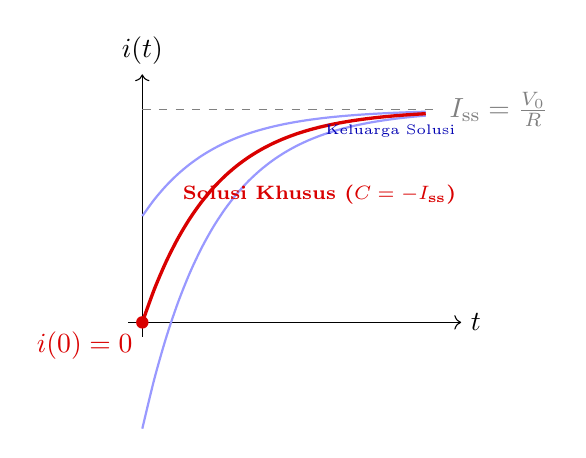
\begin{tikzpicture}[scale=0.9]
        \draw[->] (-0.2,0) -- (4.5,0) node[right] {$t$};
        \draw[->] (0,-0.2) -- (0,3.5) node[above] {$i(t)$};
        \draw[dashed, gray] (0,3) -- (4.2,3) node[right] {$I_{\text{ss}} = \frac{V_0}{R}$};
        % Kurva keluarga
        \draw[domain=0:4, smooth, blue!40, thick] plot ({\x}, {3 - 4.5*exp(-\x)});
        \draw[domain=0:4, smooth, blue!40, thick] plot ({\x}, {3 - 1.5*exp(-\x)});
        % Solusi Khusus Unik
        \draw[domain=0:4, smooth, red!85!black, very thick] plot ({\x}, {3*(1 - exp(-\x))});
        \fill[red!85!black] (0,0) circle (2.5pt) node[below left] {$i(0)=0$};
        \node[red!85!black, font=\scriptsize\bfseries] at (2.5, 1.8) {Solusi Khusus ($C = -I_{\text{ss}}$)};
        \node[blue!70!black, font=\tiny] at (3.5, 2.7) {Keluarga Solusi};
      \end{tikzpicture}%
      }
    \end{center}
  \end{columns}
\end{frame}

% FRAME 8: Derivasi Eksplisit Solusi Khusus
\begin{frame}{Derivasi Analitik Solusi Khusus Rangkaian RL}
  \textbf{Pemisahan Variabel pada PDB Rangkaian RL:}
  \begin{equation*}
    L \frac{di}{dt} = V_0 - R i \implies \frac{di}{V_0 - R i} = \frac{1}{L} dt
  \end{equation*}
  Integralkan kedua ruas persamaan secara eksplisit:
  \begin{equation*}
    \int \frac{di}{V_0 - R i} = \int \frac{1}{L} dt \implies -\frac{1}{R} \ln |V_0 - R i| = \frac{t}{L} + C_1
  \end{equation*}
  Kalikan dengan $-R$ dan eksponensialkan:
  \begin{equation*}
    \ln |V_0 - R i| = -\frac{R}{L} t - R C_1 \implies V_0 - R i(t) = A e^{-\frac{R}{L} t} \implies i(t) = \frac{V_0}{R} - \frac{A}{R} e^{-\frac{R}{L} t}
  \end{equation*}
  \begin{exampleblock}{Terapkan Kondisi Awal $i(0) = 0$}
    \begin{equation*}
      0 = \frac{V_0}{R} - \frac{A}{R} e^0 \implies \frac{A}{R} = \frac{V_0}{R} \implies \mathbf{i(t) = \frac{V_0}{R} \left(1 - e^{-\frac{t}{\tau}}\right)}, \quad \text{dengan } \tau = \frac{L}{R}
    \end{equation*}
  \end{exampleblock}
\end{frame}

% FRAME 9: Karakteristik Dinamika Transien Tau
\begin{frame}{Karakteristik Dinamika Transien \& Konstanta Waktu $\tau$}
  \begin{columns}
    \column{0.55\textwidth}
    Konstanta waktu $\tau = \frac{L}{R}$ merepresentasikan tolok ukur laju respon transien alami sistem:
    \vspace{0.15cm}
    \begin{table}[h]
      \centering
      \scriptsize
      \begin{tabular}{cccl}
        \toprule
        \textbf{Waktu $t$} & \textbf{Faktor $e^{-t/\tau}$} & \textbf{$i(t) / I_{\text{ss}}$} & \textbf{Status Rekayasa} \\ \midrule
        $0$ & $1{,}0000$ & $0\%$ & Sakelar menutup ($v_L = V_0$) \\
        $1\tau$ & $0{,}3679$ & $\mathbf{63{,}2\%}$ & Transien melesat cepat \\
        $2\tau$ & $0{,}1353$ & $86{,}5\%$ & Transien mulai melambat \\
        $3\tau$ & $0{,}0498$ & $95{,}0\%$ & Mendekati keadaan mantap \\
        $4\tau$ & $0{,}0183$ & $98{,}2\%$ & Margin galat industri $<2\%$ \\
        $5\tau$ & $0{,}0067$ & $\mathbf{99{,}3\%}$ & \textbf{Keadaan Mantap Resmikan} \\ \bottomrule
      \end{tabular}
    \end{table}

    \column{0.45\textwidth}
    \begin{alertblock}{Aturan Lima Kali Tau ($5\tau$)}
      Dalam standar rekayasa elektro, durasi waktu penyelesaian transien (\textit{settling time}) ditetapkan sebesar:
      \begin{equation*}
        t_s = 5\tau = 5 \frac{L}{R}
      \end{equation*}
      Setelah $t \ge 5\tau$, induktor bertindak sempurna sebagai \textbf{hubung singkat} ($v_L \approx 0$).
    \end{alertblock}
  \end{columns}
\end{frame}

% FRAME 10: Studi Kasus Nyata Industri (Inrush PLN)
\begin{frame}{Studi Kasus Rekayasa: Arus Inrush Trafo Gardu Induk PLN}
  \begin{columns}
    \column{0.55\textwidth}
    \begin{itemize}
      \item Pada Gardu Induk PLN (misal GI Pulau Baai 150 kV), transformator daya memiliki induktansi magnetisasi sangat besar ($L \sim \text{Henry}$) dan resistansi belitan tembaga kecil ($R \sim \text{m}\Omega$).
      \item Rasio reaktansi terhadap resistansi sangat tinggi:
      \begin{equation*}
        \frac{X}{R} \approx 30 \implies \tau = \frac{X/R}{\omega} = \frac{30}{2\pi \times 50} \approx 95{,}5\text{ ms}
      \end{equation*}
      \item Durasi peluruhan transien asimetris:
      \begin{equation*}
        t_{\text{transien}} \approx 5\tau \approx 5 \times 95{,}5\text{ ms} \approx 0{,}48\text{ detik}
      \end{equation*}
      \item Mengakibatkan \textbf{Arus Inrush} hingga $6\times - 10\times$ arus nominal.
    \end{itemize}

    \column{0.45\textwidth}
    \begin{block}{Standar Proteksi Gardu Induk}
      \textbf{IEEE Std C37.91 / SPLN:}
      Penyetelan relai diferensial transformator (\textit{relay 87T}) wajib menggunakan fitur \textit{harmonic restraint} (harmonisa ke-2) agar tidak terjadi \textit{nuisance tripping} akibat arus transien pengisian induktor trafo.
    \end{block}
  \end{columns}
\end{frame}

% FRAME 11: Worked Numerical Example
\begin{frame}{Contoh Soal Terhitung (Worked Example): Solenoida PMT}
  \textbf{Kasus Industri:} Kumparan pemutus tenaga (PMT) memiliki $R = 2{,}5\ \Omega$ dan $L = 50\text{ mH} = 0{,}05\text{ H}$. Dihubungkan ke stasiun baterai DC $V_0 = 125\text{ V}$ pada $t=0$. Induktor mula-mula kosong ($i(0)=0$).
  \vspace{0.15cm}

  \begin{columns}[t]
    \column{0.5\textwidth}
    \textbf{1. Hitung Konstanta Waktu \& Arus Mantap:}
    \begin{align*}
      \tau &= \frac{L}{R} = \frac{0{,}05\text{ H}}{2{,}5\ \Omega} = 0{,}02\text{ s} = \mathbf{20\text{ ms}} \\
      I_{\text{ss}} &= \frac{V_0}{R} = \frac{125\text{ V}}{2{,}5\ \Omega} = \mathbf{50\text{ A}}
    \end{align*}
    \textbf{2. Persamaan Arus Sesaat:}
    \begin{equation*}
      i(t) = 50 \left(1 - e^{-\frac{t}{0{,}02}}\right) = 50 (1 - e^{-50t})\quad \text{[A]}
    \end{equation*}

    \column{0.5\textwidth}
    \textbf{3. Evaluasi Nilai pada $1\tau$ dan $5\tau$:}
    \begin{itemize}
      \item $i(20\text{ ms}) = 50 (1 - e^{-1}) = \mathbf{31{,}61\text{ A}}$
      \item $i(100\text{ ms}) = 50 (1 - e^{-5}) = \mathbf{49{,}66\text{ A}}$
    \end{itemize}
    \textbf{4. Energi Medan Magnet Keadaan Mantap:}
    \begin{equation*}
      E_L = \frac{1}{2} L I_{\text{ss}}^2 = \frac{1}{2}(0{,}05)(50)^2 = \mathbf{62{,}5\text{ Joule}}
    \end{equation*}
  \end{columns}
\end{frame}

% FRAME 12: Praktikum Komputasi Julia
\begin{frame}[fragile]{Praktikum Komputasi Numerik Terbuka Berbasis Julia}
  \begin{block}{Simulasi Respon Transien Menggunakan DifferentialEquations.jl}
\begin{lstlisting}[style=juliastyle]
using DifferentialEquations, Plots

# 1. Parameter Fisik Sistem Rangkaian RL (PMT Gardu Induk)
const V0, R, L = 125.0, 2.5, 0.050    # Tegangan [V], Hambatan [Ohm], Induktansi [H]
tau = L / R; Iss = V0 / R              # tau = 0.02 s (20 ms), Iss = 50.0 A

# 2. Definisi PDB Dinamika KVL: di/dt = (V0 - R*i) / L
f_rl(i, p, t) = (V0 - R * i) / L
i0 = 0.0; tspan = (0.0, 0.12)          # Kondisi Awal & Rentang Waktu (0 s.d 6 tau)

# 3. Eksekusi Pemecah Numerik Berkecepatan Tinggi (Tsit5)
prob = ODEProblem(f_rl, i0, tspan)
sol = solve(prob, Tsit5(), reltol=1e-8, abstol=1e-8)

# 4. Plotting Hasil Analitik vs Numerik
t_vec = 0.0:0.001:0.12
i_analitik = Iss .* (1.0 .- exp.(-t_vec ./ tau))
plot(sol, label="Numerik Julia (Tsit5)", lw=2.5, color=:blue, xlabel="Waktu t [detik]", ylabel="Arus i(t) [A]")
plot!(t_vec, i_analitik, label="Solusi Analitik", lw=1.5, ls=:dash, color=:red)
savefig("transien_rl_julia.png")
\end{lstlisting}
  \end{block}
\end{frame}

% FRAME 13: Verifikasi Solusi Julia & Interpretasi
\begin{frame}{Verifikasi Hasil Komputasi Julia \& Dinamika Transien}
  \begin{columns}[t]
    \column{0.49\textwidth}
    \begin{alertblock}{Visualisasi Simulasi Tsit5()}
      \centering
      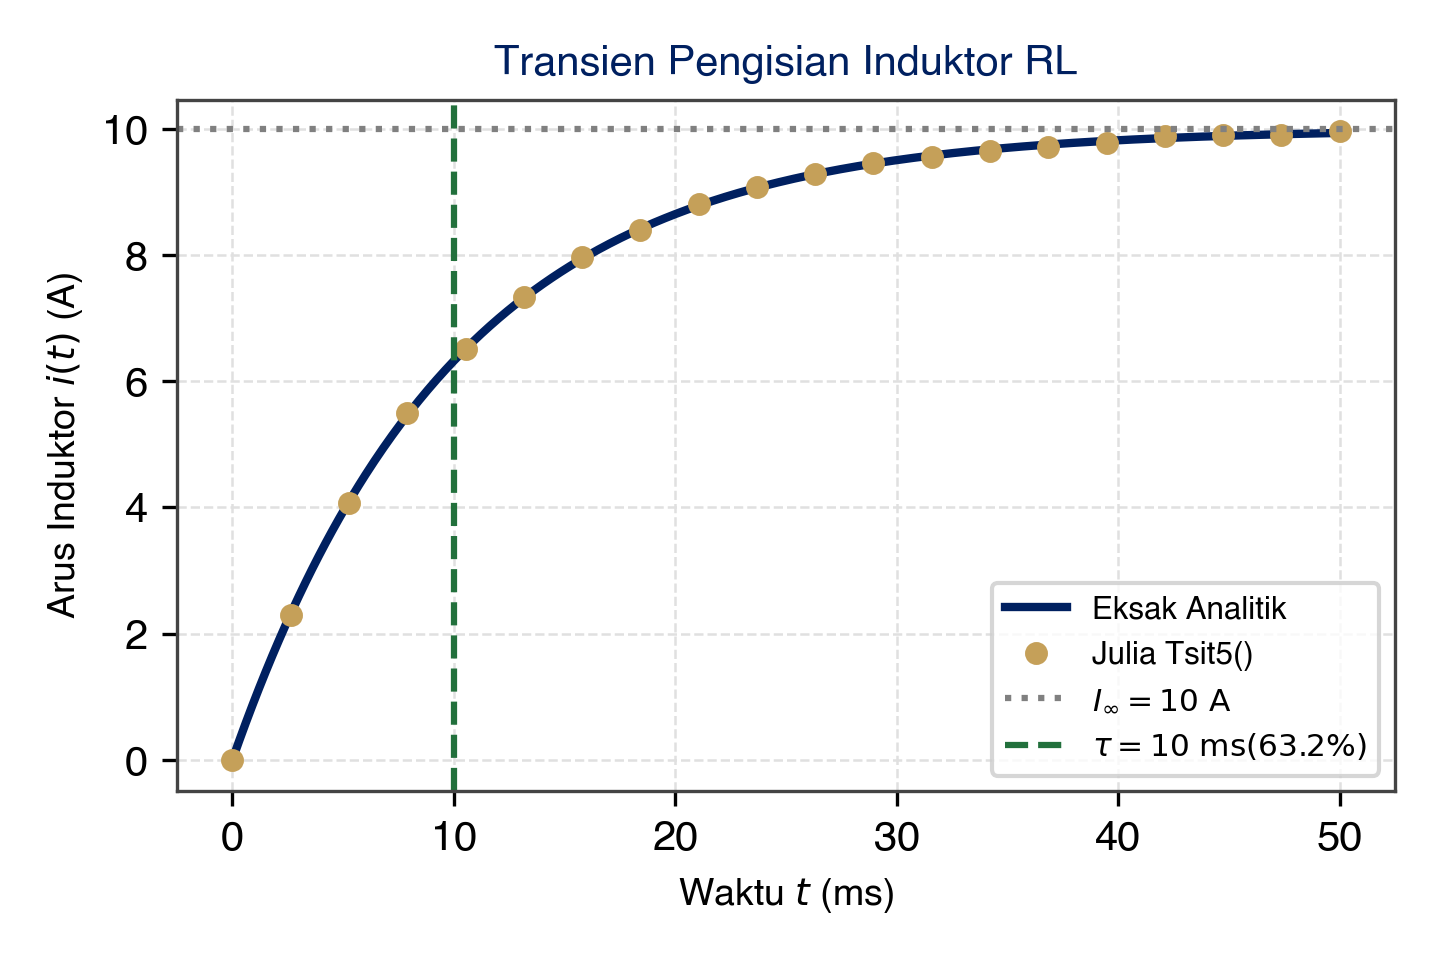
\includegraphics[width=\linewidth, height=0.38\textheight, keepaspectratio]{figures/slides/plot_ch1.png}
    \end{alertblock}
    \vspace{-0.1cm}
    \begin{exampleblock}{Intisari Dinamika Transien}
      \tiny
      Arus melaju asimtotik ke $I_{\text{ss}} = 50\text{ A}$. Pada $t = \tau = 20\text{ ms}$, arus mencapai $63{,}2\%$ ($31{,}6\text{ A}$). Pada $t = 5\tau = 100\text{ ms}$, mencapai $99{,}3\%$ ($49{,}7\text{ A}$).
    \end{exampleblock}

    \column{0.48\textwidth}
    \begin{block}{Akurasi Solver \& Laju Awal ($di/dt$)}
      \small
      \begin{enumerate}
        \item \textbf{Akurasi Sempurna:} Galat numerik \texttt{Tsit5()} terhadap analitik $< 10^{-7}\text{ A}$.
        \item \textbf{Laju Lonjakan Arus Awal ($t=0^+$):}
        Tegangan jatuh murni diserap induktor:
        \begin{equation*}
          \left.\frac{di}{dt}\right|_{t=0} = \frac{V_0}{L} = \frac{125\text{ V}}{0{,}05\text{ H}} = \mathbf{2500\text{ A/s}}
        \end{equation*}
        dan meluruh menuju nol saat tunak.
      \end{enumerate}
    \end{block}
  \end{columns}
\end{frame}

% FRAME 14: Kuis & Tantangan Evaluasi Bloom C1-C6
\begin{frame}{Kuis Konseptual Interaktif \& Evaluasi Bloom (C1--C6)}
  \begin{columns}[t]
    \column{0.52\textwidth}
    \begin{alertblock}{Peer Instruction: Uji Miskonsepsi Fisik}
      \footnotesize
      \textbf{Kasus Rekayasa:} Sakelar rangkaian RL dihubungkan ke sumber DC $V_0$. Saat sakelar ditutup pada $t=0$, mengapa arus $i(0^+) = 0$ padahal tegangan sumber $V_0$ sudah aktif penuh?
      \vspace{0.05cm}
      \begin{itemize}\setlength{\itemsep}{1pt}
        \item \textbf{[A]} Resistor $R$ memblokir aliran arus pada awal transien.
        \item \textbf{[B]} Induktor menginduksi ggl lawan $v_L = -L \frac{di}{dt}$ menentang lonjakan arus demi kekekalan fluks!
        \item \textbf{[C]} Baterai memerlukan jeda waktu melepaskan muatan.
        \item \textbf{[D]} Energi magnetik butuh hambatan luar untuk stabil.
      \end{itemize}
    \end{alertblock}

    \column{0.46\textwidth}
    \begin{block}{Tantangan Analisis \& Desain (C4--C6)}
      \footnotesize
      \begin{itemize}\setlength{\itemsep}{2pt}
        \item \textbf{C4 (Analisis):} Bandingkan disipasi kalor resistor terhadap energi tersimpan induktor ($t=0$ s.d $5\tau$).
        \item \textbf{C5 (Evaluasi):} Validasi kerja relai proteksi $30\text{ ms}$ pada arus $>75\% I_{\text{ss}}$!
        \item \textbf{C6 (Desain):} Rancang $R_{\text{snubber}}$ agar tegangan pemutusan $\le 500\text{ V}$!
      \end{itemize}
    \end{block}
  \end{columns}
\end{frame}

% FRAME 15: Rangkuman & Penutup
\begin{frame}{Rangkuman Inti Perkuliahan \& Referensi}
  \begin{exampleblock}{Intisari Perkuliahan Minggu 1}
    \begin{itemize}
      \item Dinamika sistem tenaga dan rangkaian elektrik dimodelkan oleh PDB melalui hukum KVL/KCL dan prinsip kontinuitas energi medan.
      \item Solusi umum memuat konstanta integrasi sembarang, sedangkan solusi khusus ditentukan secara tunggal oleh Nilai Awal (\textit{IVP}).
      \item Konstanta waktu $\tau = L/R$ menentukan kecepatan transien; kondisi mantap tercapai pada $t \approx 5\tau$.
    \end{itemize}
  \end{exampleblock}
  \vspace{0.2cm}
  \begin{center}
    \small \textbf{Buku Acuan Utama:} \\
    E. Kreyszig, \textit{Advanced Engineering Mathematics}, 10th ed. | W. Hayt, \textit{Engineering Circuit Analysis}. \\
    \vspace{0.3cm}
    \textbf{Tautan Modul \& Bahan Ajar}: \url{https://www.ndaratha.my.id/persamaan-diferensial/}
  \end{center}
\end{frame}

\end{document}
